\chapter{Background}
\label{chap:bg}

This chapter gives the background of \betrfs.
\betrfs is a file system based on write-optimized \bets.
Also, \betrfs adopts full-path indexing or relative-path indexing for spatial
locality.
This chapter first introduces \bets and full-path-indexed \betrfs,
showing the difficulty to perform renames efficiently on the file system level
with full-path indexing,
followed by the description of relative-path-indexed \betrfs, which has good
rename performance but taxes other operations.

\section{\bets}
\label{sec:bet}

\bets~\citep{bet,betlogin} are \btrees, augmented with buffers in non-leaf
nodes.
New writes are injected as messages into the buffer of the root node of a \bet.
When a node's buffer becomes full, messages are flushed from that node's buffer
to one of its children's buffers.
The leaves of the \bet store key/value pairs, as in a \btree.
Point and range queries on a \bet must check related messages in the buffers
along the root-to-leaf path, as well as key/value pairs in the leaves.

\begin{table}[t]
    \centering
    \begin{tabular}{c | c c c}
        \hline
        Data Structure & Insert & Point Query & Range Query \\
        \hline
        \hline
        \btree & $O(log_{B}{N})$ & $O(log_{B}{N})$ & $O(log_{B}{N} + k/B)$\\
        \hline
        \bet & $O({log_{B}{N}}/{\varepsilon B^{1 - \varepsilon}})$ & $O({log_{B}{N}}/{\varepsilon})$ & $O({log_{B}{N}}/{\varepsilon} + k/B)$ \\
        \hline
        \bet ($\varepsilon=0.5$) & $O(log_{B}{N}/{\sqrt{B}})$ & $O(log_{B}{N})$ & $O(log_{B}{N} + k/B)$ \\
        \hline
    \end{tabular}
    \caption[The asymptotic IO costs of \btrees and \bets]{\label{tab:betbtree}
        The asymptotic IO costs of \btrees and \bets.}
\end{table}

\bets are asymptotically faster than \btrees, as summarized in
Table~\ref{tab:betbtree}.
Consider a \btree with $N$ key/value pairs and in which each node can hold
$B$ keys
(for simplicity, assume keys have constant size and that the value associated
with each key has negligible size).
The tree has fanout $B$, so its height is $O(log_{B}{N})$.
Inserts and point queries need to fetch all nodes along the root-to-leaf path,
resulting in $O(log_{B}{N})$ IOs.
A range query for $k$ key/value pairs requires $O(log_{B}{N} + k/B)$ IOs.

For comparison, a \bet with node size $B$ has fanout $B^{\varepsilon}$, where
$0 < \varepsilon \leq 1$.
Therefore, pivot keys in a non-leaf node consume $B^{\varepsilon}$ space and
the remaining $(B - B^{\varepsilon})$ space is used for buffers.
As a result, the \bet has height $O(log_{B}{N}/\varepsilon)$.
A point query fetches all nodes along the root-to-leaf path with
$O(log_{B}{N}/\varepsilon)$ IOs and a range query for $k$ key/value pairs
requires $O({log_{B}{N}}/{\varepsilon} + k/B)$ IOs.
On the other hand, the cost of an insert consists of injecting the message into
the root node with $O(1)$ IO and flushing the message down at each level.
In each flush, \bets has $O(B - B^{\varepsilon})$ messages and $B^{\varepsilon}$
children.
Thus, at leave one child can receive at least
$O((B - B^{\varepsilon})/B^{\varepsilon}) = O(B^{1 - \varepsilon})$ messages.
Therefore, the amortized cost of an insert in one flush is
$O(1/B^{1 - \varepsilon})$.
As the insert must be flushed $O(log_{B}{N}/\varepsilon)$ times, the amortized
cost of the insert is $O({log_{B}{N}}/{\varepsilon B^{1 - \varepsilon}})$.
A \bet with $\varepsilon = 1$ is equivalent to a \btree.
And if $\varepsilon = 1/2$, the point and range query costs of the \bet
become $O(log_{B}{N})$ and $O(log_{B}{N} + k/B)$, which is the same as a \btree,
but the insert cost becomes $O(log_{B}{N}/{\sqrt{B}})$, which is faster by a
factor of $\sqrt{B}$.

One important change in \bets from \btrees is the asymmetric IO costs for
point queries and inserts.
In \btrees, if an application wants to update the old value associated with a
key, it performs a point query to get the old value and then issues an insert
with the updated value.
Because both operations take $O(log_{B}{N})$ IOs, the total cost remains
$O(log_{B}{N})$.
However, in \bets, the query cost is $O(log_{B}{N}/\varepsilon)$ IOs while the
insert cost is $O({log_{B}{N}}/{\varepsilon B^{1 - \varepsilon}})$.
Performing a query before an insert degrades the total cost to
$O(log_{B}{N}/\varepsilon)$ IOs.

To avoid this read-before-write problem, \bets support ``upsert'' operations.
An upsert injects a message with the key and a delta into the buffer of the root
node.
When the upsert message is flushed to the leaf, it updates the old value
associated with the key with a user-specified function and the delta in the
message.
With upsert messages, queries need to compute value on the fly.
However, this doesn't change the IO costs of queries.
On the other hand, updating an old value becomes as fast as an insert.

\section{Full-path-indexed \betrfs}
\label{sec:fpi}

\begin{figure}
    \centering
    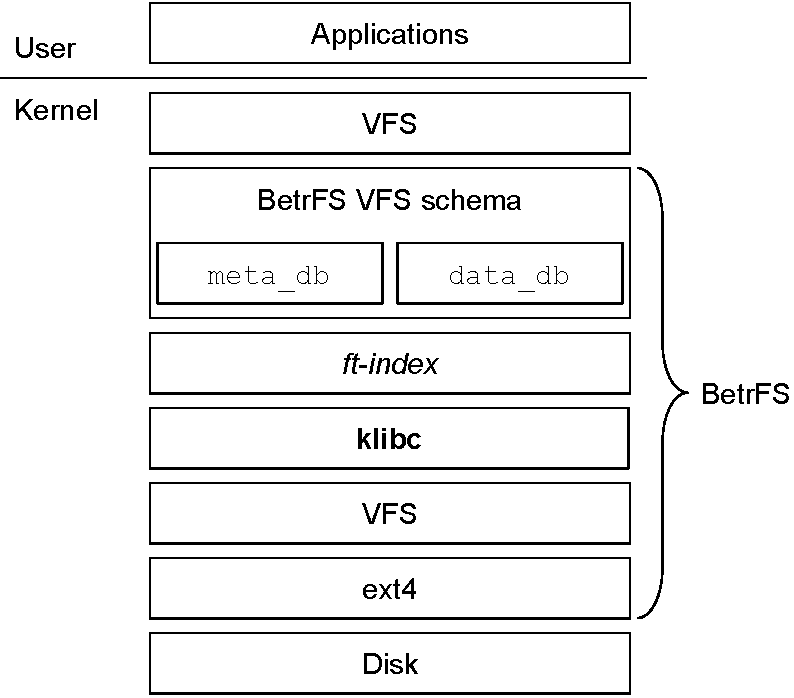
\includegraphics{fig/betrfs}
    \caption[The \betrfs architecture]{\label{fig:betrfs}
        The \betrfs architecture.}
\end{figure}

\betrfs~\citep{betrfs1,betrfs1tos} is a Linux in-kernel file
system built upon \fti~\citep{fti}, a key/value store that implements \bets and
exposes a key/value interface similar to BerkelyDB.
The architecture of \betrfs is shown in Figure~\ref{fig:betrfs}.
\betrfs interacts with \fti through point operations, such as \texttt{put},
\texttt{get} and \texttt{del}, as well as range queries with cursors
(\texttt{c\_get} with DB\_SET\_RANGE and DB\_NEXT).
\betrfs also uses the transaction interface of \fti to execute multiple
operations atomically.
A redo log and periodic checkpoints (every 60 seconds) in \fti ensure that
changes can be made persistent on disk.

\Fti cannot be integrated into a Linux kernel module easily because
it is a userspace library that assumes libc functions and system calls.
\betrfs has a shim layer called \klibc that implements all functions \fti
requires.
Through this way, \betrfs can incorporate \fti into the kernel module without
modifying code in \fti.

\betrfs uses two key/value indexes to store the metadata and data in the file
system.
One \texttt{meta\_db} maps full-paths to \texttt{struct stat} structures.
Another \texttt{data\_db} maps (full-path and block number) to 4KB blocks.
When the VFS (Virtual File System) needs metadata, \betrfs queries
the \texttt{meta\_db} with the full-path and constructs the corresponding inode
from the \texttt{struct stat}.
Likewise, when a dirty inode needs to be written, the \texttt{struct stat} is
assembled from the inode and written to the \texttt{meta\_db} with the
full-path key.
Blocks of a file are fetched and written by the full-path and the indexes of
blocks.
Although other block granularity is possible, 4KB is the natural block size
because it is the same as the page size in the Linux page cache.

\betrfs can write to a block without fetching the old block to memory, avoiding
expensive read-before-write described in Section~\ref{sec:bet}.
Conventional file systems must read the old block from the disk to the page
cache before writing to that block (a complete overwrite can be done without
fetching the old block, but it is not implemented in any file system).
However, \bets have asymmetric read and write costs, so read-before-write should
be avoided.
In \betrfs, if the corresponding block is not in memory, an upsert message,
which describes the offset, length and content of this write, is injected into
the \bet.
When this message is flushed to the leaf, the change is applied to the old
block.

Full-path indexing ensures locality even with file system aging~\citep{betrfs3}.
After \betrfs fetches one block of a file from the disk, all nodes along the
root-to-leaf path are present in memory.
And with full-path indexing, all keys under one directory are contiguous in the
keyspace, which means a subsequent fetch of some other block in the same file or
another file under than same directory is likely to be resolved in memory,
which significantly increases performance and IO efficiency.

The first implementation of \betrfs (\betrfsOne) shows great random write
performance.
Recursive greps run 3.77x faster than in the best standard file system.
File creation runs 12.54x faster.
Small, random writes to a file run 68.24x faster~\citep{betrfs1tos}.

However, namespace operations have predictably miserable performance in
\betrfsOne.
Deleting and renaming a Linux source directory takes 46.14 and 21.17 seconds,
resepctively, because the file system has to call one or more key/value store
operations for each key.
The deleting problem is fixed by a range-delete message that nullifies all
messages within a range, but the renaming problem remains diffcult.

\section{Relative-path-indexed \betrfs}
\label{sec:rpi}

\begin{figure}
    \begin{subfigure}{.5\textwidth}
        \centering
        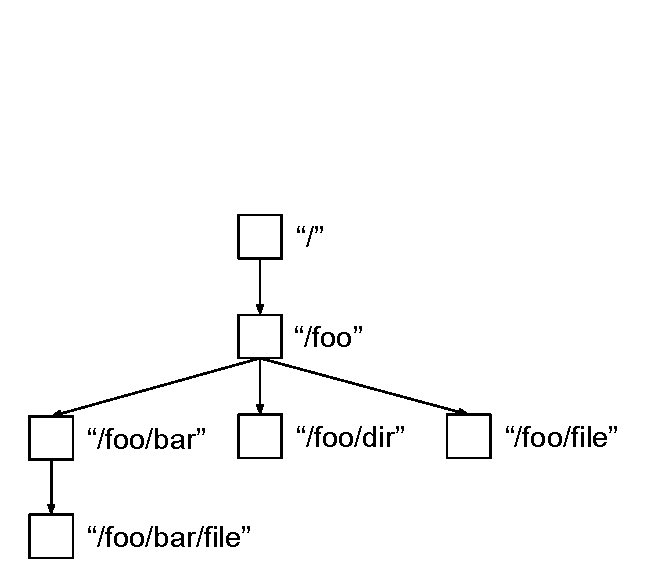
\includegraphics[width=.9\linewidth]{proposal/fig/FPI}
        \caption{\label{subfig:FPI} Full-path indexing.}
    \end{subfigure}
    \begin{subfigure}{.5\textwidth}
        \centering
        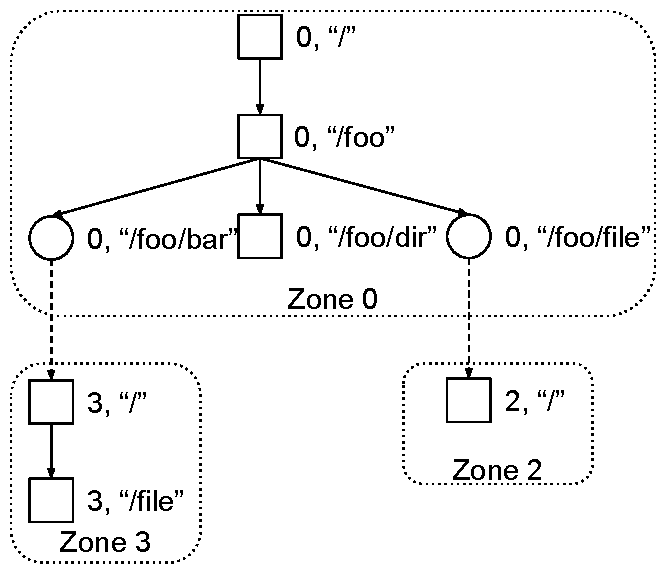
\includegraphics[width=.9\linewidth]{proposal/fig/RPI}
        \caption{\label{subfig:RPI} Relative-path indexing.}
    \end{subfigure}
    \caption[Full-path indexing and relative-path indexing]{\label{fig:FPIRPI}
        Full-path indexing and relative-path indexing.}
\end{figure}

Relative-path-indexed \betrfs~\citep{betrfs2,betrfs2tos} backed away from
full-path indexing and introduced relative-path indexing,
which is also called zoning.
Relative-path indexing partitions the directory hierarchy into zones.
Each zone has a zone ID (the root zone has zone ID 0), which is analogous to an
inode number, and a single root file or directory.
All file or directory in a zone is indexed relative to the zone root.
If the file or directory is the root of another zone, the entry contains that
zone ID to redirect queries.

Figure~\ref{fig:FPIRPI} shows an example of the same directory hierarchy under
full-path indexing and relative-path indexing.
In Figure~\ref{subfig:RPI}, when querying the key/value store for file
``/foo/file'' with key (0, ``/foo/file''), the file system gets a special value
indicating it is the root of Zone 2.
Subsequently, the file system queries the key/value store with key (2, ``/'')
and gets the right value.
Similary, the file system notices the key for directory ``/foo/bar'' is
(3, ``/'').
Therefore, when querying for file ``/foo/bar/file'', it uses key (3, ``/file'').

\begin{figure}[t]
    \centering
    \begin{tikzpicture}
        \begin{axis}[
            xlabel={Files created},
            ylabel={Throughput (files/sec)},
            xmin=0,
            xmax=3000000,
            ymin=10,
            ymax=50000,
            mark repeat=10,
            xtick={0,1000000,2000000,3000000},
            xticklabels={0,1M,2M,3M},
            ytick={10000,20000,30000,40000,50000},
            yticklabels={10k,20k,30k,40k,50k},
            grid=major,
            scaled x ticks=false,
            scaled y ticks=false,
            legend cell align=left,
            transpose legend,
            height=.5\linewidth,
            width=.8\linewidth,
        ]
        \addTokubenchZonePlot{betrfs3};
        \addTokubenchZonePlot{betrfs3-max};
        \end{axis}
    \end{tikzpicture}
    \caption[Zone maintainance cost in TokuBench]{Cumulative file creation
        throughput during the Tokubench benchmark (higher is better).
        Compared to \betrfsThree with one zone, \betrfsThree has a sudden
        performance drop because of zone splitting.}
    \label{fig:tokuzone}
\end{figure}

Relative-path indexing tries to balance locality and rename performance through
a target zone size.
Larger zone size means better locality because full-path indexing is still
maintained within the zone.
Smaller zone size imposes a lower bound on rename latency
because no rename needs to mutate more key/value pairs than in a zone.

\betrfsTwo adopts relative-path-indexing with a default zone size 128KiB.
Relative-path indexing made renames on \betrfsTwo almost as fast as inode-based
file system and recursive-directory traversals almost as fast as \betrfsOne.

However, relative-path indexing also imposes zone maintainance costs on other
file system operations.
For instance, in Figure~\ref{fig:tokuzone},
two-thirds of the way through the TokuBench benchmark,
\betrfsThree (\betrfsThree is \betrfsTwo with some bug fixes) shows a sudden,
precipitous drop in cumulative throughput for small file creation,
because the file system performs a huge amount of zone splitting.
On the contrary, \betrfsThree with an infinite zone size (marked as \betrfsThree
with one zone) has a smooth curve throughout the benchmark.

Furthermore, relative-path indexing also has bad worst-case performance.
It is possible to construct arrangements of nested directories that will each
reside in their own zone.
Reading a file in the deepest directory will require reading one zone per
directory (each withits own I/O).
Such a pathological worst case is not possible with full-path indexing in a
\bet, and an important design goal for \betrfs is keeping a reasonable bound on
the worst cases.

\section{Summary}

\betrfs is a general file system designed for all operations, with a particular
focus on random writes and localtiy.
The underlying data strucutre, \bets, performs random writes faster than \btrees
by casading writes in batches.
The full-path indexing schema of \betrfsOne ensures good locality, while making
renames slow.
The relative-path indexing schema of \betrfsTwo enables fast renames,
but imposes additional costs on other operations.

